% !TEX root = main.tex

\section{索引与散列} % Chap 11
\subsection{基本概念}
\begin{definition}[聚集索引]
包含记录的文件按照某个搜索码指定顺序排序,则该搜索码对应的索引称为聚集索引(clustering index),也被称为主索引(primary)。
但注意并不是建立在主码上的索引。
若搜索码指定的顺序与文件中记录的物理顺序不同,则称为非聚集索引。
\end{definition}

\begin{figure}[H]
\centering
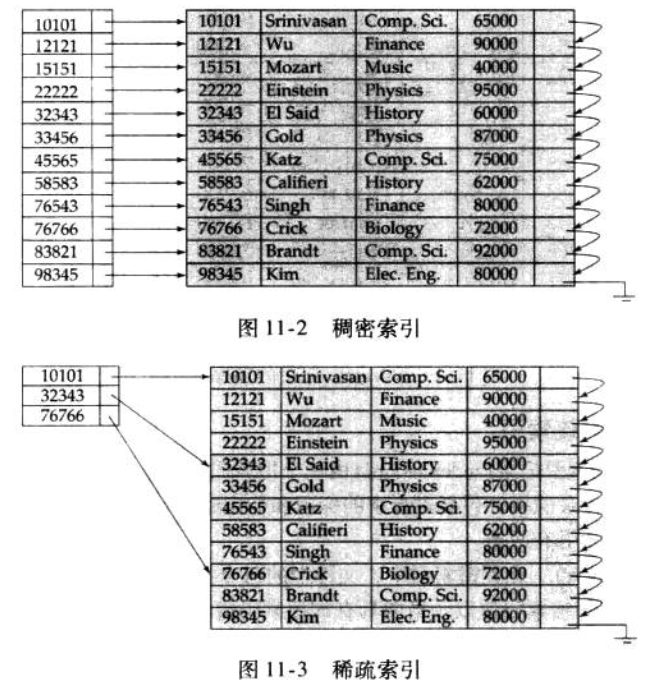
\includegraphics[width=0.6\linewidth]{fig/dense_sparse_indexing.png}
\end{figure}

通过建造多级稀疏索引,来减少访问时间。

\subsection{B+树索引文件}
B+树索引采用平衡树结构,树根到树叶的每条路径长度相同。

$m$-阶B树满足以下性质:
\begin{itemize}
	\item 所有叶子结点都必须在同一层
	\item 除了根结点外的结点都至少有$\lceil m/2\rceil -1$个关键字,最多$m-1$个关键字
	\item 除了根结点外的非叶子节点都至少有$\lceil m/2\rceil$个孩子
	\item 每个结点有$m$个指针,$m-1$个键值
	\item 所有结点键值都必须以升序排序
\end{itemize}

而B+树则是将所有关键字存储在叶子结点,其他结点作为索引,并且为每个叶子结点增加一个链指针。
\begin{figure}[H]
\centering
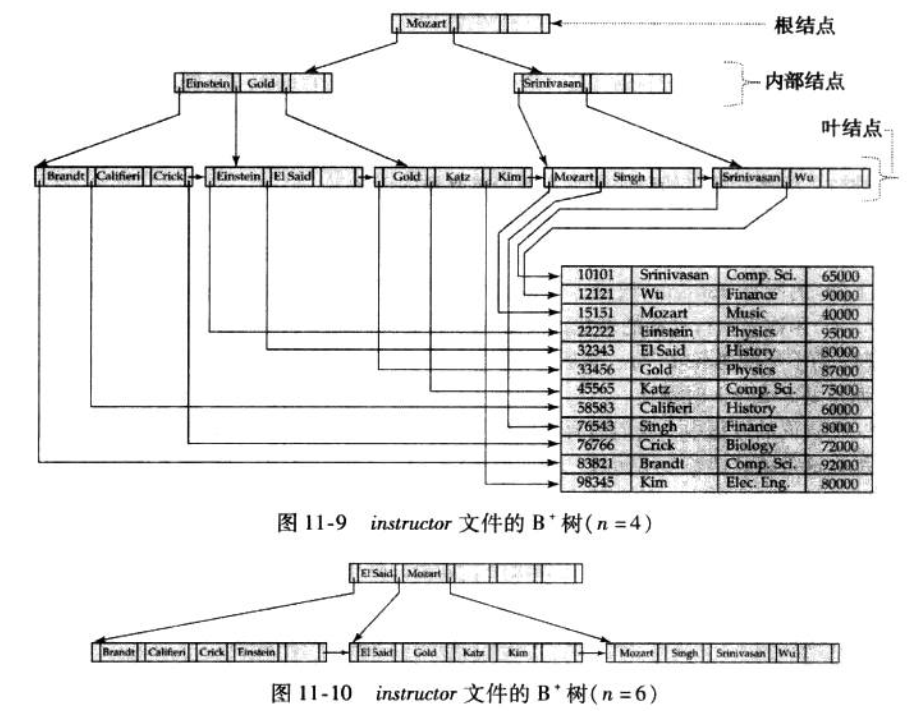
\includegraphics[width=0.6\linewidth]{fig/bp-tree.png}
\end{figure}

插入和删除操作都会造成结点的分裂。

\subsection{静态散列}
散列(hash)函数应该满足:
\begin{itemize}
	\item 分布均匀:为每个桶分配同样数量的搜索码值
	\item 分布随机:不应与搜索码的任何外部可见排序相关
\end{itemize}

线性探查法(probing):插入到下一个有空间的桶

下例的散列函数为ID各位数字之和对8取模
\begin{figure}[H]
\centering
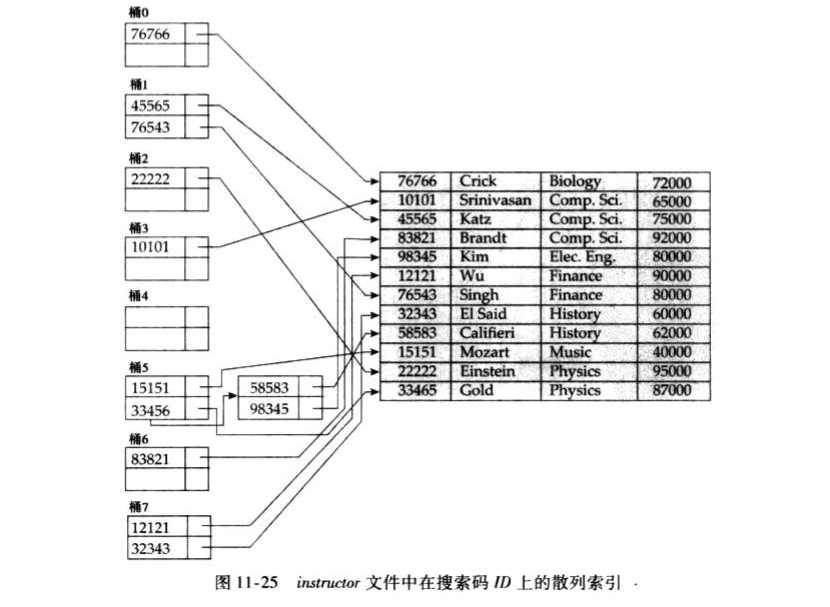
\includegraphics[width=\linewidth]{fig/hash_index.png}
\end{figure}

\subsection{动态散列}
当数据库增大或缩小时,可扩充散列(extendable hashing)可通过桶的分裂或合并来适应数据库大小变化。

但缺点在于查找涉及一个附加的间接层,系统在访问桶本身之前必须先访问桶地址表。

\subsection{位图索引}
某个属性存在则设为1,否则置0。
\begin{figure}[H]
\centering
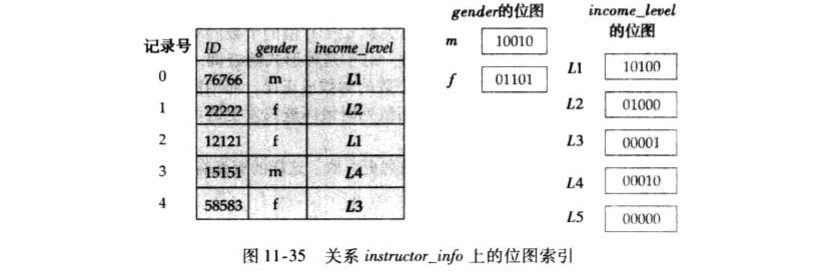
\includegraphics[width=0.9\linewidth]{fig/bitmap.png}
\end{figure}